% !TEX root = ../Projektdokumentation.tex
\subsection{Ressourcen}

\subsubsection{Personal}
Die Arbeiten werden durch eine Person durchgeführt. Der Stundenansatz ist auf 120 CHF angesetzt und gilt für die folgenden Berechnungen. Bei den Berechnungen werden die Aufwände der Experten nicht berücksichtigt.

%\begin{itemize}
%	\item Alle Projektmitarbeiter mit ihren Funktions-, Tätigkeits- und Kompetenzbereichen.
%	\item Welche Mittel, Infrastruktur werden benötigt?
%	\item Was steht zur Verfügung?
%	\item Mess-, Versuchs- und Testgeräte müssen genau protokolliert werden!
%\end{itemize}
%\subsubsection{Arbeitskräfte}
%Die benötigten Arbeitskräfte sind wiefolgt definiert:
%\newline
%\newline
%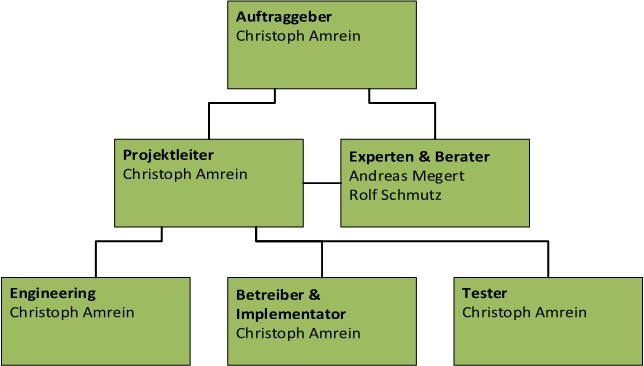
\includegraphics[scale=0.8]{Bilder/Projektorganisation.jpg}}

\subsubsection{Phasenaufwände und Kosten}

\begin{table}[H]
\centering
\begin{tabular}[t]{p{4cm}p{4cm}p{4cm}}
\hline
\rowcolor{heading}\textbf{Phase} & \textbf{Personalaufwand \newline in Stunden} & \textbf{ Kosten \newline in CHF} \\\hline
Initialisierung & 30 & 3'600 \\\hline
Konzept & 50 & 6'000 \\\hline
Realisierung & 142 & 17'040 \\\hline
Einführung & 22 & 2'640 \\\hline 
Periodische Arbeiten & 25 & 3'000 \\\hline
Reserve & 25 & 3'000 \\\hline
\textbf{Total} & \textbf{294} & \textbf{35'280}  \\\hline
\end{tabular}
\caption{Phasenaufwände und Kosten}
\end{table}

\subsubsection{Budget}
Für das Projekt sind folgende Kosten einberechnet.
\begin{table}[H]
\centering
\begin{tabular}[t]{p{1cm}p{5cm}p{2cm}}
\hline
\rowcolor{heading}\textbf{Nr.} & \textbf{Verwendungszweck} & \textbf{Budget \newline in CHF} \\\hline
1 & Apéro & 150 \\\hline
2 & Drucken \& Binden & 60 \\\hline
3 & Zusätzliche Beschaffungen & 390 \\\hline
\textbf{} & \textbf{Total} & \textbf{600}  \\\hline
\end{tabular}
\caption{Projektbudget}
\end{table}

\subsubsection{Sachmittel}
Es werden folgende Komponenten für die Durchführung der Arbeit benötigt. Alle Komponenten wurden ausserhalb des Projektes beschafft und werden nicht in den Projektkosten berücksichtigt:


\begin{table}[H]
\centering
\begin{tabular}[t]{p{1cm}p{1.2cm}p{6.5cm}p{6.5cm}}
\hline
\rowcolor{heading}\textbf{Nr.} & \textbf{Anzahl} & \textbf{Komponenten} & Modell / Spezifikationen\\\hline
1 & 40 & Mini Computer & Raspberry PI 3 Model B+\\\hline
2 & 1 & Schaltnetzteil & RSP-750-5, Mean Well\\\hline
3 & 1 & Midi Tower & Corsair Crystal 570X RGB\\\hline
4 & 1 & USB zu TTL Serial-Kabel & Adafruit USB zu TTL Seriel Kabel, 75cm (Kabel) \\\hline
5 & 40 & Ethernetkabel & FTP Cat.5e Patchkabel \\\hline
6 & 1 & Switch & TL-SL3452 48-Port 10/100, TP-Link \\\hline
7 & 1 & Datenspeicher & Synology NAS DS218\\\hline
8 & * & Diverses, Kabel, Distanzbolzen, \newline Kabelschuhe & *\\\hline
\end{tabular}
\caption{Sachmittel}
\end{table}
* Anzahl und Hertseller unbekannt. Die Artikel wurden in lokalen Baumärkten eingekauft